\documentclass{article}
\usepackage[utf8]{inputenc}
\usepackage[margin=1in]{geometry}
\usepackage{csquotes}

\usepackage{algorithm}
\usepackage[noend]{algpseudocode}

\usepackage{tikz}
\usetikzlibrary{trees}

\title{$2^n$ Dynamic Programming}
\author{Lawrence Wang and Kevin Geng\footnote{Highly inspired by Samuel Hsiang's lecture from last year.}}
\date{2 December 2016}

\begin{document}

\maketitle

\section{Problem statement}

(USACO December 2014, Gold Problem 1: Guard Mark)

Farmer John and his herd are playing frisbee. Bessie throws the frisbee down the field, but it's going straight to Mark the field hand on the other team!  Mark has height $H$ ($1 \leq H \leq 1,000,000,000$), but there are $N$ cows on Bessie's team gathered around Mark ($2 \leq N \leq 20$)\footnote{Whenever you see $N \leq 20$, an exponential-time solution is likely!}. They can only catch the frisbee if they can stack up to be at least as high as Mark.  Each of the N cows has a height, weight, and strength. A cow's strength indicates the maximum amount of total weight of the cows that can be stacked above her.

Given these constraints, Bessie wants to know if it is possible for her team to build a tall enough stack to catch the frisbee, and if so, what is the maximum safety factor of such a stack.  The safety factor of a stack is the amount of weight that can be added to the top of the stack without exceeding any cow's strength.

\section{$N!$ solution}

A naive solution would be to recursively construct all permutations of the $N$ cows, where on each level of recursion we append a cow to the bottom of the stack. This solution has complexity $O(N!)$, which is too slow for the input size. 

% Make this less horrible pls
% Also we might want to include a picture of the tree and circle the subsets that are being recomputed
To see why the naive solution performs so badly, we can examine the search tree for a small case (say $N=4$). Notice how if we select any subset of cows, there is only one optimal permutation that maximizes the height and minimizes the total weight. For example, there will be one optimal way to order cows $A$, $B$, and $C$. However, we notice that in the search tree, there are multiple paths originating from the root of length three that consist of cows $A$, $B$, and $C$.

If we want to check all solutions that begin with some permutation of $A$, $B$, and $C$ and end with a fourth cow $D$, then we only need to consider the optimal ordering of $A$, $B$, and $C$. We can do this because we are trying to add $D$ to the bottom, and the total weight of the three cows will not change.

\begin{figure}[h!]
\centering
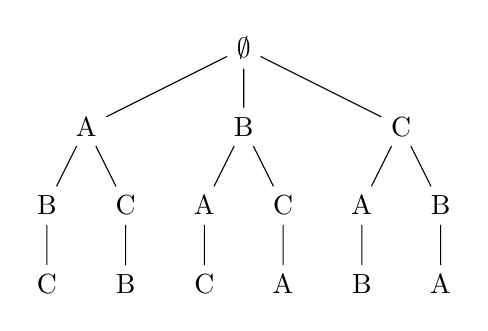
\begin{tikzpicture}[level distance=1cm,
    level 1/.style={sibling distance=2cm},
    level 2/.style={sibling distance=1cm}]
    \node {$\emptyset$}
        child {node {A}
            child {node {B}
              child {node {C}}
            }
            child {node {C}
              child {node {B}}
            }
        }
        child {node {B}
            child {node {A}
                child {node {C}}
            }
            child {node {C}
                child {node {A}}
            }
        }
        child {node {C}
            child {node {A}
                child {node {B}}
            }
            child {node {B}
                child {node {A}}
            }
        };
\end{tikzpicture}
\caption{All permutations of $A$, $B$, and $C$.}
\end{figure}

\section{$2^n$ solution}

Thus, we wish to constructively generate subsets of the $N$ cows rather than permutations, since each subset encapsulates an optimal permutation. This leads us to develop \textit{subset DP}, which allows us to perform DP over $2^n$ possible subsets instead of $n!$ permutations.

The base case of our dynamic programming formulation are subsets containing one element. For our recurrence relation, we consider a subset $S$, which has some optimal ordering that has already been computed. In order to increase the size of this subset, we consider adding a cow that is not already in $S$ to the bottom of $S$. This is possible whenever the strength of the cow to be added is greater than the total weight of $S$. 

Adding cows to an existing subset takes $O(N)$ since in the worst case we must check every cow to add. Since there are $O(2^N)$ total subsets of the $N$ cows (why?), the overall time complexity is $O(N 2^N)$. While this may still appear to be very slow, it is sufficient for the input limits and is a significant speed-up from the naive $O(N!)$ solution.   

% Insert pseudocode

\section{Bit Masking}

While the above solution theoretically solves the problem, it may at first appear too clumsy to implement. Fortunately, we can compactly and elegantly represent subsets using a bit string: there is a bijective mapping between a bit string of size $N$ and subsets of a size $N$ set. Specifically, we can represent each subset as a sequence of bits, where each bit corresponds with a cow. If a bit is set to one, then the corresponding cow is in the subset, while if a bit is set to zero, then the cow is not in the subset.

We can manipulate bits using bit masking operations: namely, and, or, xor, not, left shift, and right shift.\footnote{Throwback to ACSL!} For the most part, however, we only need to know a few operations:

\begin{enumerate}
    \item \verb@num | (1 << i)@ to set bit $i$
    \item \verb|num & ~(1 << i)| to clear bit $i$
    \item \verb|num ^ (1 << i)| to toggle bit $i$
    \item \verb|num & (1 << i)| to test bit $i$
\end{enumerate}

%We can easily manipulate these bits using a number of bit masking operations (THROWBACK TO ACSL). These include AND, OR, XOR, and negation. AND is frequently used to set a bit to 0, while OR is used to set a bit to 1. Furthermore, XOR is used to toggle a bit on or off. We can also select a specific bit using the left and right shift operators, which are effectively equivalent to multiplying and dividing by two respectively. While these are the primary uses of bit operations, they also have a number of other uses, such as in Fenwick trees. 

% Maybe insert a table here, similar to how Sam did it

\begin{algorithm}[H]
\caption{$2^n$ solution}
\begin{algorithmic}
    \For{$i \gets 0 \dots 2^n-1$}
    \Comment{$i$ represents the subset $S$}
        \State $dp(index) \gets \infty$
        \Comment{safety factor}
        \ForAll{$j \in S$}
        \Comment{such that bit $j$ is set in $i$}
            \State $prev \gets i-2^j$
            \Comment{clear bit $j$}
            \State $alt \gets min(dp(prev), strength(j)-\sum_{k \in S \setminus \{j\}} weight(j))$
            \Comment{calculate new safety factor}
            \If{$dp(i) < alt$}
                \State $dp(i) \gets alt$
            \EndIf
        \EndFor
    \EndFor
\end{algorithmic}
\end{algorithm}

This pseudocode finds the maximum safety factor for any subset. There are, however, a few more complications in the problem that need to be handled. Specifically, we need to keep track of the total weight and height of each subset to keep the runtime $O(n*2^n)$, as well as determine whether any subset actually exceeds the requested height. Completing the implementation of these details is left as an exercise to the reader.

\pagebreak

\section{More problems}

\begin{enumerate}
    \item USACO 2015 January, Gold Problem 2: Movie Mooving
    
    Bessie is out at the movies.  Being mischievous as always, she has decided to hide from Farmer John for $L$ ($1 \leq L \leq 100,000,000$) minutes, during which time she wants to watch movies continuously. She has $N$ ($1 \leq N \leq 20$) movies to choose from, each of which has a certain duration and a set of showtimes during the day.  Bessie may enter and exit a movie at any time during one if its showtimes, but she does not want to ever visit the same movie twice, and she cannot switch to another showtime of the same movie that overlaps the current showtime.
    
    Help Bessie by determining if it is possible for her to achieve her goal of watching movies continuously from time $0$ through time $L$.  If it is, determine the minimum number of movies she needs to see to achieve this goal (Bessie gets confused with plot lines if she watches too many movies).

    \item USACO 2014 February, Gold Problem 2: Cow Decathlon
    \item USACO 2013 January, Gold Problem 2: Island Travels
\end{enumerate}
\end{document}
